\documentclass{article}

% IMPORT PACKAGES
\usepackage{graphicx}
\graphicspath{{images/}}
\usepackage{blindtext}
\usepackage[T1]{fontenc}
\usepackage[latin9]{inputenc}
\usepackage[a4paper]{geometry}
\geometry{verbose,tmargin=2cm,bmargin=2cm,lmargin=1cm,rmargin=1cm}
\setlength{\parskip}{\smallskipamount}
\setlength{\parindent}{0pt}
\usepackage{array}
\usepackage{mathtools}
\usepackage{dsfont}
\usepackage{amsmath}
\usepackage{amssymb}
\usepackage{lmodern}
\usepackage{eqlist}
\usepackage{babel}
\usepackage{multicol}
% BLOCKS
\usepackage{beamerarticle}
\usepackage[most]{tcolorbox}
%	COMMON COLORS
\definecolor{_light_green}{rgb}{0.36, 0.84, 0.36}
\definecolor{_light_grey}{rgb}{0.90, 0.90, 0.90}
\definecolor{_white}{rgb}{1.0, 1.0, 1.0}
\definecolor{_blue}{rgb}{0.0, 0.0, 1.0}
\definecolor{_light_blue}{rgb}{0.7, 0.9, 1.0}
%	DEFINE BOXES
\newtcolorbox{_block}[1][]{
    colbacktitle=_light_grey,		% title background
    coltitle=black,					% title color
    titlerule=0pt,
    colback=white!50!_light_grey,	% body background
    boxrule=0.4pt,					% content-frame padding (or frame width)
    colframe=black!20!_light_grey,	% frame color
    left=0mm,						% content and title left padding
    arc=0.5pt,						% border-radius
    title={#1},
}
\newtcolorbox{_example}[1][]{
    colbacktitle=_light_green,
    coltitle=black,
    titlerule=0pt,
    colback=white!60!_light_green,
    boxrule=0pt,
    colframe=white,
    left=0mm,
    arc=0.5pt,
    title={#1},
}
\newtcolorbox{_note}[1][]{
    colbacktitle=_light_blue,
    coltitle=black,
    titlerule=0pt,
    colback=white!60!_light_blue,
    boxrule=0pt,
    colframe=white,
    left=0mm,
    arc=0.5pt,
    title={#1},
}
\newtcolorbox{_block_emph}[1][]{
    enhanced,
    frame hidden,
    borderline west={2.0pt}{0pt}{blue!60!white},
    opacityframe=0.0,
    colback=blue!4!white,
    left=2mm,
    arc=0.5pt,
    title={#1},
}

% \usepackage{subfiles}
% \subfile{}

% DOCUMENT

\begin{document}

% short title:
%   \part*{}
%   \part[]{}

\title{CS3237 Introduction to Internet of Things \\ Group 4 Report}
\author{Lai Yu Heem, Pinkl Constantin Maxime, Teo Chuan Kai, Wong Chee Hong, Thomm Leon Felix}
\maketitle

% changing sections enumeration style
% styles: \arabic{} \alph{} \Alph{} \roman{} \Roman{}
\renewcommand\thesection{\arabic{section}}
\renewcommand\thesubsection{\thesection.\alph{subsection}}

\section{Abstract}

\textbf{Tino}

\section{Introduction}

\textbf{Tino}

\section{Solution Approach}

\textbf{Chuan Kai}

\subsection{Architecture overview}

\begin{multicols}{2}

Physically, the system consists of two components: the \textit{cloud} and the \textit{buoy(s)}, whereas a buoy can be further divided into \textit{WeMOS} and \textit{Phone}. 

The WeMOS collects most of the data of interest (temperature, movement, water turbidity). It then sends collected records to the phone via WiFi, which extends it and does some timestamp modification. The phone also serves as a gateway and forwards the records to the server running in the cloud.

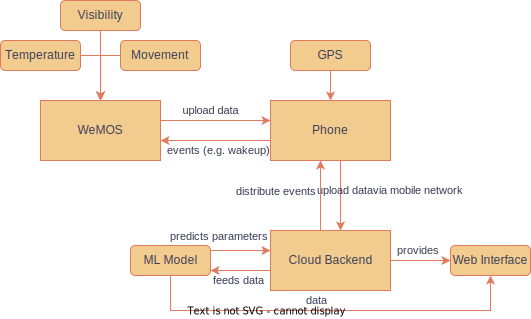
\includegraphics[width=8cm]{report/resources/architecture.png}

\end{multicols}

\subsection{Buoy Hardware}

\subsection{Phone applications}

\textbf{Tino}

\subsection{Server-side}

\textbf{Chuan Kai}

\subsection{ML model and application}

\textbf{Yu Heem}

\subsection{Front-End}

\textbf{Chuan Kai}

\section{Implementation Details}

\subsection{Turbidity sensor}

\textbf{Chee Hong}

\subsection{Waterproofing}

\textbf{Chee Hong}

\subsection{Power modes and sampling frequencies}

\textbf{Leon}

\subsection{$\text{I}^2\text{C}$ Communication}

\textbf{Leon}

\subsection{Buoy-Server}

\textbf{Chuan Kai}

\subsection{Data collection}

\textbf{Tino}

\section{Experimental Evaluation}

\subsection{Model accuracy}

\textbf{Chuan Kai}

\subsection{Power consumption estimates}

\textbf{Leon}

\section{Challenges and Outlook}

\subsection{Phone reliance}

\textbf{Tino}

\subsection{Data bottleneck}

\textbf{Yu Heem}

\subsection{Statistical methods}

\textbf{Chee Hong}

\subsection{Other use-cases}

\textbf{???}

\subsection{...}

\end{document}